\documentclass{beamer}
\mode<presentation>{
	\usetheme{Madrid}
}

\usepackage{graphics}
\usepackage{tikz}
\graphicspath{{./pictures}}
\usepackage[T1]{fontenc}
\usepackage{polski}
\title[]{Analiza porównawcza zastosowań tradycyjnych oraz wariacyjnych autoenkoderów}
\institute[UMCS]
{
	Uniwersytet Marii Curie Skłodowskiej
	\medskip
}
\author{Filip Ręka}
\date{\today}

\begin{document}
% 1
	\begin{frame}
		\titlepage
	\end{frame}

	\begin{frame}
		\tableofcontents
	\end{frame}
% 2
	\begin{frame}
		\frametitle{Cele}
		\section{Cel}
		\begin{itemize}
			\item Opisanie budowy modelu autoenkodera oraz jego zastosowań
			\item Przestawienie problemów tradycyjnej architektury w celu generacji nowych danych
			\item Opisanie budowy wariacyjnego autoenkodera
			\item Generacja danych, podobnych do tych, na których model został wytrenowany
		\end{itemize}
	\end{frame}
% 3
	\begin{frame}
		\frametitle{Autoenkoder}
		\section{Autoenkoder}
		Autoenkoder składa się z dwóch części: enkodera oraz dekodera. Obie z nich są w pełni połączonymi sieciami neuronowymi, które również są połączone pomiędzy sobą. Zadaniem enkodera jest zakodowanie jego wejścia do kodu o stałej długości, co jest osiągane przez architekturę warstw, w której każda następna ma mniej neuronów. Dekoder jest częścią, która z kodu, próbuje odwzorować zakodowane dane. Cały autoenkoder dostaje na warstwę wejściową oraz wyjściową te same dane, przez co jego sposób uczenia jest nazywany częściowo nadzorowanym. 
	\end{frame}

% 4
	\begin{frame}
		\frametitle{Architektura autoenkodera}
		\begin{figure}
			\centering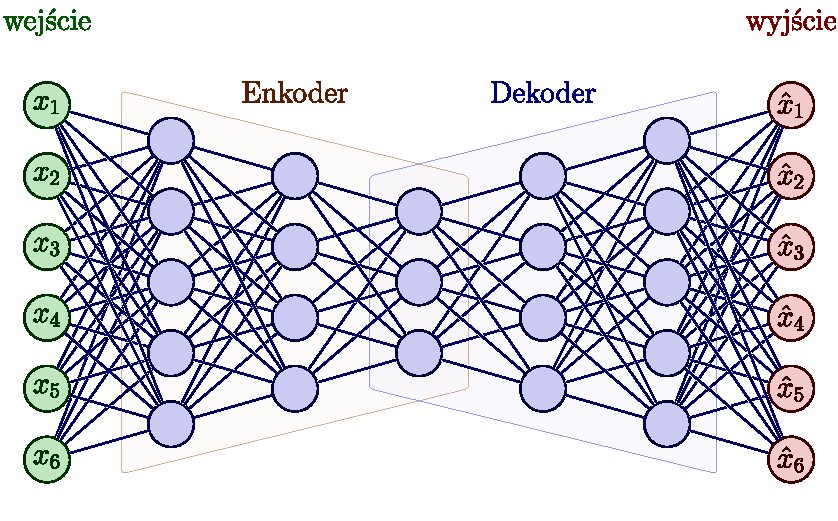
\includegraphics[width=10cm]{tikzae.pdf}
			\caption{Przykładowa architektura modelu}
		\end{figure}
	\end{frame}

% 5
	\begin{frame}
		\frametitle{Zastosowania autoenkodera}
		\subsection{Zastosowania autoenkodera}
		Głównym zadaniem autoenkodera jest kompresja. Funkcję tą, można zastosować do redukcji wymiarów czy odszumiania danych, co zawdzięczamy temu, że kompresja dokonywana przez model jest stratna. W ten sposób autoenkoder, musi zachować w kodzie jak najwięcej istotnych elementów. 
		\vspace{-0.3cm}
		\begin{figure}
			\centering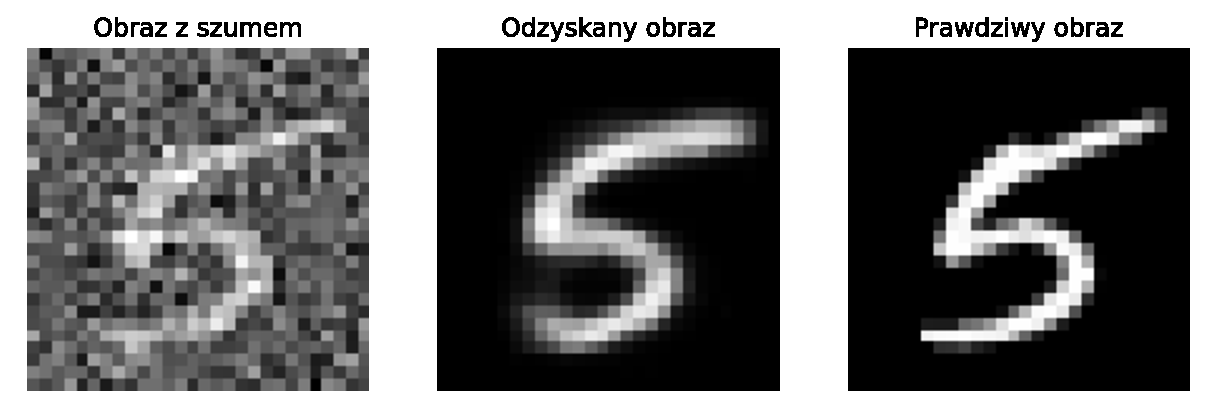
\includegraphics[width=7cm]{denoisingae.pdf}
			\caption{Rekonstrukcja obrazu przy pomocy autoenkodera}
		\end{figure}
		\vspace{-0.5cm}
		Zaletą używania autoenkoderów w celu redukcji wymiarów w przeciwieństwie do metody analizy składowych głównych (PCA) jest ich możliwość nauki nieliniowych zależności pomiędzy wymiarami.
	\end{frame}

% 6
	\begin{frame}
		\frametitle{Problem generacji danych}
		\subsection{Problem generacji danych}
		Aby wygenerować nowe dane, podobne do tych na których model został wytrenowany, potrzebujemy ściśle określonej dystrybucji według której punkty, reprezentujące skompresowane wejście, są rozłożone. Tradycyjna architektura nie zapewnia nam tego faktu, ani takich wymagać jak kompletności oraz ciągłości przestrzeni kodu. 
	\end{frame}
		
% 7
	\begin{frame}
		\frametitle{Wariacyjny autoenkoder}
		\section{Wariacyjny autoenkoder}
		Wariacyjny autoenkoder rozwiązuje problemy z generacją nowych danych tradycyjnego modelu. Aby model był generacyjny, potrzebujemy ściśle ustalonej dystrybucji, z której losujemy punkty, na podstawie których generujemy dane. W przypadku modelu VAE, jest to wielowymiarowy rozkład normalny, opisywany za pomocą wektorów odchylenia standardowego $\sigma$ oraz średniej $\mu$. Następnie z tych dystrybucji losujemy punkty $z$, które traktujemy jako kod, na podstawie, których rekonstruujemy wejście modelu.
	\end{frame}

	\begin{frame}
		\frametitle{Budowa wariacyjnego autoenkodera}
		\begin{figure}
			\centering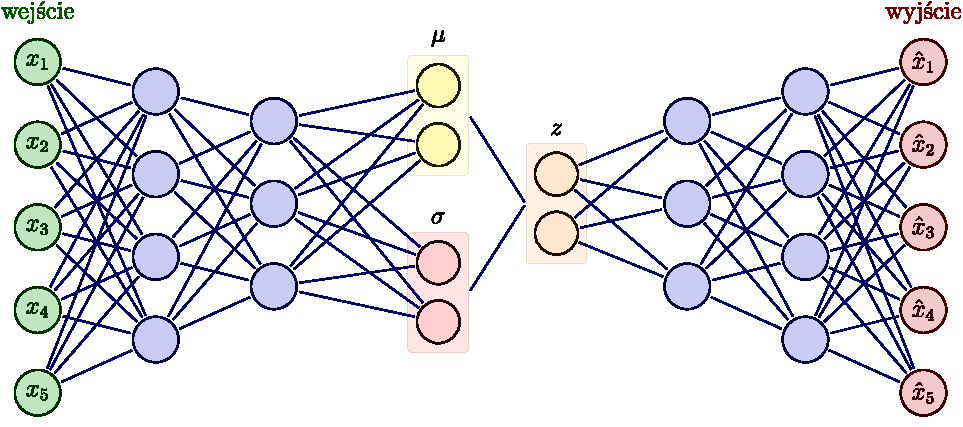
\includegraphics[width=10cm]{tikzvae.pdf}
			\caption{Przykład architektury modelu}
		\end{figure}
	\end{frame}

	\begin{frame}
		\subsection{Generacja nowych danych}
		\frametitle{Generacja nowych danych}
		Posiadając enkoder, który generuje kod należący co ściśle określonej dystrybucji, można wybierając z niej losowe punkty generować dane. 
		
		\begin{figure}
			\centering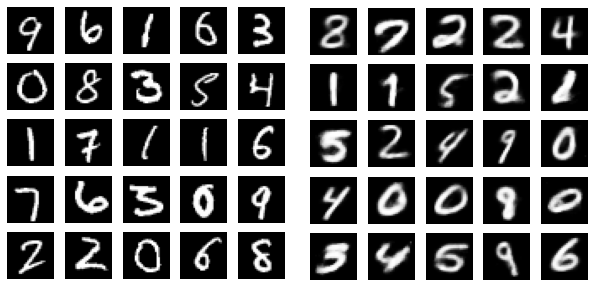
\includegraphics{vaegeneracja.png} 
			\caption{Po lewej stronie są dane ze zbioru, a po prawej wygenerowane}
		\end{figure}
	
	Powyższy przykład przedstawia generację na podstawię zbioru danych MNIST.
		
	\end{frame}

	\begin{frame}
		\begin{center}
			\huge Dziękuje za uwagę!
		\end{center}
	\end{frame}
\end{document}